\documentclass[convert]{standalone}
\usepackage{amsmath}
\usepackage{tikz}
\usepackage{mathdots}
\usepackage{yhmath}
\usepackage{cancel}
\usepackage{color}
\usepackage{siunitx}
\usepackage{array}
\usepackage{multirow}
\usepackage{amssymb}
\usepackage{gensymb}
\usepackage{tabularx}
\usepackage{booktabs}
\usetikzlibrary{fadings}
\usetikzlibrary{patterns}
\usetikzlibrary{shadows.blur}
\usetikzlibrary{shapes,snakes}


\begin{document}
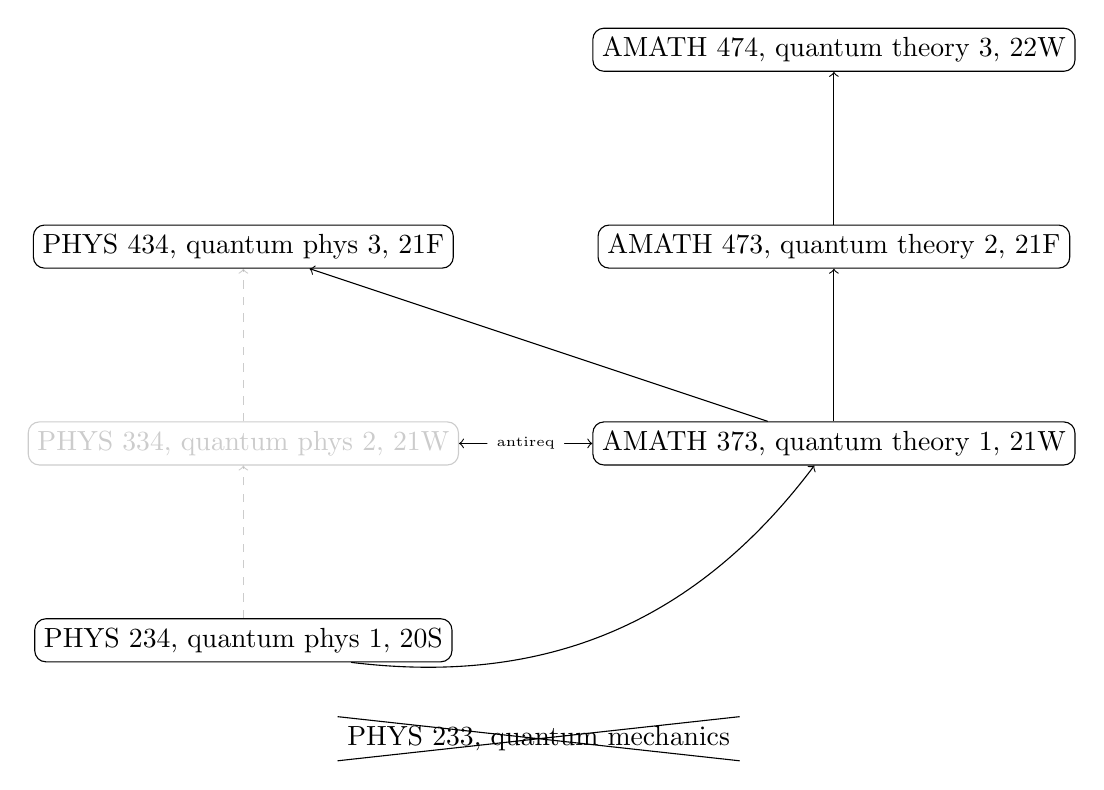
\begin{tikzpicture}[scale=0.5,every node/.style={draw, rectangle, rounded corners}]

\node[cross out]  at (7.5,-2.5) {PHYS 233, quantum mechanics};
\node (p1) at (0,0) {PHYS 234, quantum phys 1, 20S};
\node[opacity=0.2] (p2) at (0,5) {PHYS 334, quantum phys 2, 21W};
\node (p3) at (0,10) {PHYS 434, quantum phys 3, 21F};

\node (a1) at (15, 5) {AMATH 373, quantum theory 1, 21W};
\node (a2) at (15, 10) {AMATH 473, quantum theory 2, 21F};
\node (a3) at (15, 15) {AMATH 474, quantum theory 3, 22W};

%\draw [<->] (p2) edge (a1);
\path[<->] (p2) edge node[ draw=none,fill=white, pos=0.5] {\tiny antireq} (a1);

\path[->, dashed, opacity=0.2] (p1) edge (p2);
\path[->, dashed, opacity=0.2] (p2) edge (p3);
\path[->, bend right] (p1) edge (a1);
\path[->] (a1) edge (p3);
\path[->] (a1) edge (a2);
\path[->] (a2) edge (a3);
\end{tikzpicture}
\end{document}
